\documentclass{article}

\usepackage{../swiftnav}
\usepackage{../swiftnav_tikz}
\usepackage{tikz-timing}
\usetikztiminglibrary{advnodes}

\rhead{Swift Navigation NAP}

\usepackage{draftwatermark}
\SetWatermarkLightness{0.85}
\SetWatermarkText{Preliminary}
\SetWatermarkScale{4}

\usetikzlibrary{calc,fit,matrix,chains}

\usetikzlibrary{shapes.geometric,shapes.arrows,decorations.pathmorphing}
\usetikzlibrary{scopes,positioning,arrows}

\version{2.2.0}
\title{Swift Navigation NAP\\(Navigation Acceleration Peripheral)}
\author{Swift Navigation}
\date{\today}

\begin{document}

\newcommand{\samplebits}{3}
\newcommand{\feclkfreq}{16.368}
\newcommand{\samplesperms}{16368}
\newcommand{\spiclkfreqs}{8.184, 16.368, 32.736, 49.104, 65.472, and 81.840 MHz}

\newcommand{\numtrackchans}{12}

\newcommand{\acqntaps}{16}
\newcommand{\acqfreqmult}{3}
\newcommand{\acqfreqmhz}{49.104}
\newcommand{\acqspeed}{80}
\newcommand{\acqlength}{49104}
\newcommand{\acqms}{3}

\newcommand{\cwfreqmult}{4}
\newcommand{\cwfreqmhz}{65.472}
\newcommand{\cwgranularityhz}{15}
\newcommand{\cwlength}{65472}
\newcommand{\cwms}{4}

\newcommand{\iirntaps}{5}
\newcommand{\iirfreqmhz}{81.840}
\newcommand{\iirnbits}{10}

\newcommand{\numcorrelators}{88}
\newcommand{\numgmaccs}{2.88}

\maketitle

\raggedcolumns
\begin{multicols}{2}

\section*{Overview}

The Swift Navigation NAP (Navigation Acceleration Peripheral) is a multi-function hardware accelerator, implemented using a Xilinx Spartan 6 FPGA (Field-Programmable Gate Array), for the lowest levels of signal processing in the Swift Navigation GNSS Receiver. It groups correlators into channels with specific purposes while allowing the user a large amount of control and flexibility.

The SwiftNAP includes \numtrackchans\ tracking channels with low level interfaces, each containing 6 channels : one each for early I, early Q, prompt I, prompt Q, late i, and late q (half chip spacing). It includes one serial search acquisition correlator that searches \acqntaps\ consecutive code phases in parallel (quarter chip spacing), at \acqfreqmult x the sample clock, giving a \acqspeed x acquisition speed over real time. Finally, it includes a spectrum power analyzation correlator for detecting continuous wave interference, and a \iirntaps\ tap IIR filter for continuous-wave rejection between the frontend samples and the acquisition and tracking channels.
\columnbreak

\section*{Features}
\begin{itemize} 
  \bulletnoindent
  \setlength{\itemsep}{4pt}
  \item \samplebits\ bit samples
  \item \feclkfreq\ MHz sample clock frequency
  \item \numcorrelators\ correlators
  \item \numtrackchans\ tracking channels / 6 correlators each
  \item 1/\acqspeed\ real time acquisition channel / \acqntaps\ correlators
  \item Dedicated CW (continuous-wave) detection channel
  \item \iirntaps -tap IIR filter for CW filtering
  \item Low level control
\end{itemize}

\renewcommand{\labelitemi}{\color{alt}\footnotesize{$\bullet$}}
\begin{itemize}
    \setlength{\itemsep}{0pt}
    \item Acquisition channel searches user specified single carrier frequency / \acqntaps\ consecutive code phases in parallel, giving quick, flexible cold/warm start capability
    \item Tracking channels with user updated code/carrier frequencies, giving high degree of phase control
    \item Continuous-wave detection channel with \cwgranularityhz\ Hz granularity reports spectrum power at user specified frequency 
    \item IIR filter's \iirnbits-bit signed coefficients set and updated directly by user
\end{itemize}

\pagebreak
\tableofcontents
\pagebreak

\end{multicols}

\section{Block Diagram}
\begin{center}
  \begin{tikzpicture}[point/.style={circle,inner sep=0pt,minimum size=2pt,fill=red},
                      tip/.style={->,shorten >=1pt}]

    \tikzstyle{antenna} = [draw,isosceles triangle,minimum width=5mm,shape border rotate=300,color=red]
    \tikzstyle{block} = [draw, fill=orange!20, rectangle, text width=1.5cm, minimum height=2.0cm, minimum width=2.0cm, line width=0.5pt]
    \def\filterSS{\node[block]{};\draw[line width=1pt] (-4mm,-2mm) to[in=220,out=40] (4mm,-2mm) 
                                                        (-4mm,0mm) to[in=220,out=40] (4mm,0mm) 
                                                        (-4mm,2mm) to[in=220,out=40] (4mm,2mm)
                                                       (-1mm,-1mm) to (1mm,1mm);}
    \tikzstyle{connection_matrix} = [matrix of nodes,
          column sep=0.45cm,
          row sep=0.45cm,
          anchor=center,
          nodes={anchor=center}] 

    \tikzstyle{blocks_matrix} = [matrix of nodes,
          column sep=0.25cm,
          row sep=0.25cm,
          anchor=center,
          nodes={anchor=center}] 
    
    %Draw blocks
    \matrix[blocks_matrix] (blocks) at (0,0) {
       %First row
       \node[below] (from frontend) {From Frontend}; & \node[minimum width=1.0cm] {}; & & \filterSS & & \\
       %Second row
       & & \node[block] (cw) {CW \ \ \ Detection Channel}; & & \node[block] (acq) {Acquisition Channel}; & \node[block] (trackfront) {Tracking Channels}; & \node[minimum width=2cm] {}; & \\
       %Third row
       & & \node[] (cw nodes center) {}; & \node[] (filter nodes center) {}; & \node[] (acq nodes center) {}; & \node[] (track nodes center) {}; & \node[] (nap stm arrows center) {}; & \node[minimum height=3cm] (to stm center) {}; \\
    };
    %"To STM" label
    \node[right of=to stm center,node distance=1.5cm] {To/From STM};
    %Assign filter to blocks-1-4
    \coordinate (filter_west) at (blocks-1-4.west);
    \coordinate (filter_east) at (blocks-1-4.east);
    \coordinate (filter_south) at (blocks-1-4.south);
    \coordinate (filter_north) at (blocks-1-4.north);

    %CW signal connections
    \matrix[connection_matrix] (cw nodes south) at (cw.south) {
      |[coordinate]| & |[coordinate]| & |[coordinate]| & |[coordinate]| \\};
    \matrix[connection_matrix] (cw nodes below) at (cw nodes center) {
       & |[coordinate]| & & & & |[coordinate]| \\
       & & & & |[coordinate]| & \\
       & & & |[coordinate]| & & \\
       & & |[coordinate]| & & & \\
       & |[coordinate]| & & & & \\
       |[coordinate]| & & & & & \\};

    %Filter signal connections
    \matrix[connection_matrix] (filter nodes south) at (filter_south) {
      |[coordinate]| & |[coordinate]| & |[coordinate]| & |[coordinate]| \\};
    \matrix[connection_matrix] (filter nodes below) at (filter nodes center) {
       & |[coordinate]| & & & & |[coordinate]| \\
       & & & & |[coordinate]| & \\
       & & & |[coordinate]| & & \\
       & & |[coordinate]| & & & \\
       & |[coordinate]| & & & & \\
       |[coordinate]| & & & & & \\};

    %Acq signal connections
    \matrix[connection_matrix] (acq nodes south) at (acq.south) {
      |[coordinate]| & |[coordinate]| & |[coordinate]| & |[coordinate]| \\};
    \matrix[connection_matrix] (acq nodes below) at (acq nodes center) {
       & |[coordinate]| & & & & |[coordinate]| \\
       & & & & |[coordinate]| & \\
       & & & |[coordinate]| & & \\
       & & |[coordinate]| & & & \\
       & |[coordinate]| & & & & \\
       |[coordinate]| & & & & & \\};

    %Tracking signal connections
    \matrix[connection_matrix] (track nodes south) at (trackfront.south) {
      |[coordinate]| & |[coordinate]| & |[coordinate]| & |[coordinate]| \\};
    \matrix[connection_matrix] (track nodes below) at (track nodes center) {
       & & & & & |[coordinate]| \\
       & & & & |[coordinate]| & \\
       & & & |[coordinate]| & & \\
       & & |[coordinate]| & & & \\
       & |[coordinate]| & & & & \\
       |[coordinate]| & & & & & \\};

    %STM signal connections
    \matrix[connection_matrix] (nap nodes) at (nap stm arrows center) {
      |[coordinate]| \\ |[coordinate]| \\ |[coordinate]| \\ |[coordinate]| \\};
    \matrix[connection_matrix] (stm nodes) at (to stm center) {
      |[coordinate]| \\ |[coordinate]| \\ |[coordinate]| \\ |[coordinate]| \\};

    %Label for filter
    \draw (filter_north) node[above, name=filter label, inner sep=1mm] {IIR Filter};

    %Other tracking channel boxes, then redraw original
    \draw let \p1=(trackfront) in ($(\x1+3mm, \y1+3mm)$) node[block,text width=1.7cm] (trackback) {};
    \draw let \p1=(trackfront) in ($(\x1+1.5mm, \y1+1.5mm)$) node[block,text width=1.7cm] (trackmid) {};
    \draw (trackfront) node[block,text width=1.7cm] (trackfront) {Tracking Channels};

    %Frontend clock initial segment and frontend data connections
    \path let \p0=(from frontend),\p1=(filter_west) in 
       coordinate(clock sig first seg orig) at ($(\x0,\y1) + (15mm,-6mm)$)
       coordinate(clock sig first seg dest) at ($(\x0,\y1) + (20mm,-6mm)$)
       coordinate(frontend data orig) at ($(\x0,\y1) + (15mm,0mm)$);
    \draw[>-,color=black!100,thick] (clock sig first seg orig) -- node[right,very near end,font=\scriptsize,text width=1cm] {Frontend\\Clock} (clock sig first seg dest);
    \draw[-,color=black!100,thick] (clock sig first seg dest) |- node[name=clock sig downward] {} (cw nodes below-5-2);
    \draw[>->,thick] (frontend data orig) -| node[above,font=\scriptsize] {3 bit samples} (cw);
    \path let \p0=(frontend data orig),\p1=(cw) in coordinate (filter data sig orig) at ($(\x1,\y0)$);
    \draw[->,thick] (filter data sig orig) -- (filter_west);

    %Data signal connections
    \draw[->,thick] (filter_east) -| (acq);
    \path let \p0=(filter_east),\p1=(acq),\p2=(trackmid),\p3=(trackback.north) in 
      coordinate (track data sig orig) at ($(\x1,\y0)$)
      coordinate (track data sig dest) at ($(\x2,\y3)$);
    \draw[->,thick] (track data sig orig) -| node[above,near start,font=\scriptsize] {1 bit filtered} (track data sig dest);

    %Clock signal multipliers
    \node[block] (cw multiplier) at (cw nodes below-1-2) [minimum width=5mm,minimum height=5mm,text width=3mm] {x\cwfreqmult};
    \node[block] (filter multiplier) at (filter nodes below-1-2) [minimum width=5mm,minimum height=5mm,text width=3mm] {x\iirntaps};
    \node[block] (acq multiplier) at (acq nodes below-1-2) [minimum width=5mm,minimum height=5mm,text width=3mm] {x\acqfreqmult};

    %Interrupt line connections
    \definecolor{irqcolor}{RGB}{225,0,0}
    \draw[<-,color=irqcolor,thick] (cw nodes below-4-3) -- (cw nodes south-1-2);
    \draw[<-,color=irqcolor,thick] (filter nodes below-4-3) -- (filter nodes south-1-2);
    \draw[<-,color=irqcolor,thick] (acq nodes below-4-3) -- (acq nodes south-1-2);
    \draw[<-,color=irqcolor,thick] (track nodes below-4-3) -- (track nodes south-1-2);
    \draw[-,color=irqcolor,thick] (cw nodes below-4-3) -- (nap nodes-3-1);
    \draw[>->,color=irqcolor,thick] (nap nodes-3-1) -- node[above,font=\scriptsize,color=black] {IRQ} (stm nodes-3-1);
    %Timing strobe line connections
    \definecolor{strbcolor}{RGB}{0,165,0}
    \draw[->,color=strbcolor,thick] (cw nodes below-3-4) -- (cw nodes south-1-3);
    \draw[->,color=strbcolor,thick] (filter nodes below-3-4) -- (filter nodes south-1-3);
    \draw[->,color=strbcolor,thick] (acq nodes below-3-4) -- (acq nodes south-1-3);
    \draw[->,color=strbcolor,thick] (track nodes below-3-4) -- (track nodes south-1-3);
    \draw[-,color=strbcolor,thick] (cw nodes below-3-4) -- (nap nodes-2-1);
    \draw[<-<,color=strbcolor,thick] (nap nodes-2-1) -- node[above,font=\scriptsize,color=black] {Timing Strobe} (stm nodes-2-1);
    %SPI 
    \definecolor{spicolor}{RGB}{0,0,225}
    \draw[<->,color=spicolor,thick] (cw nodes below-2-5) -- (cw nodes south-1-4);
    \draw[<->,color=spicolor,thick] (filter nodes below-2-5) -- (filter nodes south-1-4);
    \draw[<->,color=spicolor,thick] (acq nodes below-2-5) -- (acq nodes south-1-4);
    \draw[<->,color=spicolor,thick] (track nodes below-2-5) -- (track nodes south-1-4);
    \draw[-,color=spicolor,thick] (cw nodes below-2-5) -- (nap nodes-1-1);
    \draw[<->,color=spicolor,thick] (nap nodes-1-1) -- node[above,font=\scriptsize,color=black] {SPI} (stm nodes-1-1);
    %Clock signal connections
    \draw[-,color=black!100,thick] (cw nodes below-5-2) -- (cw multiplier);
    \draw[->,color=black!100,thick] (cw multiplier) -- (cw nodes south-1-1);
    \draw[-,color=black!100,thick] (filter nodes below-5-2) -- (filter multiplier);
    \draw[->,color=black!100,thick] (filter multiplier) -- (filter nodes south-1-1);
    \draw[-,color=black!100,thick] (acq nodes below-5-2) -- (acq multiplier);
    \draw[->,color=black!100,thick] (acq multiplier) -- (acq nodes south-1-1);
    \draw[->,color=black!100,thick] (track nodes below-5-2) -- (track nodes south-1-1);
    \draw[-,color=black!100,thick] (cw nodes below-5-2) -- (nap nodes-4-1);
    \draw[>->,color=black!100,thick] (nap nodes-4-1) -- node[above,font=\scriptsize,color=black] {Frontend Clock} (stm nodes-4-1);

  \end{tikzpicture}
  \captionof{figure}[ToC entry]{SwiftNAP Block Diagram}
\end{center}

\begin{multicols}{2}

%Change section header font size
\titleformat*{\section}{\color{alt}\normalfont\Large\bfseries}
\section{Motivation}

A typical GPS receiver signal flow is shown below:

\begin{center}
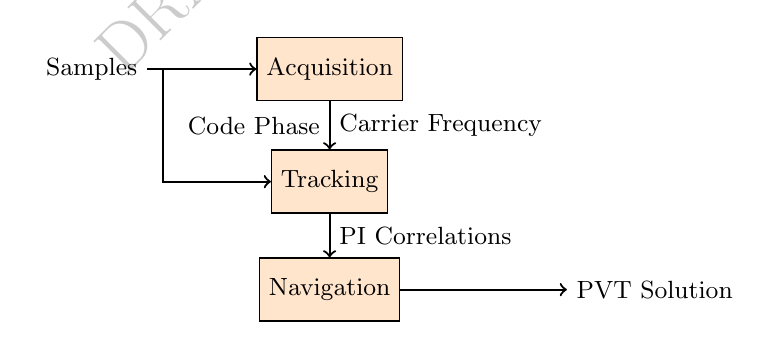
\begin{tikzpicture}

  \tikzstyle{block} = [draw, fill=orange!20, rectangle, minimum height=0.8cm, line width=0.5pt]

  \matrix (foo) [matrix of nodes, column sep=0.2cm,row sep=0.05cm, anchor=center, 
                 nodes={anchor=center,font=\small}]
  {
    \node[left] (samples) {Samples}; & \node[coordinate] (input) {}; & \node[block] (acq) {Acquisition}; &  \\ %First Row
     & & \node[left] {Code Phase}; \node[right] {Carrier Frequency}; &  \\ %Second Row
     & & \node[block] (track) {Tracking}; & \\ %Third Row
     & & \node[left] {}; \node[right] {PI Correlations}; &  \\ %Fourth Row
     & & \node[block] (nav) {Navigation}; & \node[right] (output) {PVT Solution}; \\ %Fifth row
  };

  \draw[-,color=black!100,thick] (samples) -- (input);
  \draw[->,color=black!100,thick] (input) -- (acq);
  \draw[->,color=black!100,thick] (input) |- (track);
  \draw[->,color=black!100,thick] (acq) -- (track);
  \draw[->,color=black!100,thick] (track) -- (nav);
  \draw[->,color=black!100,thick] (nav) -- (output);
  
\end{tikzpicture}
\captionof{figure}[ToC entry]{Typical GPS Receiver Signal Flow}
\end{center}

The acquisition and tracking blocks perform essentially the same DSP operation - a correlation of
the incoming baseband samples with a locally generated carrier and spreading code, as represented
by the below equation:

\normalfont\footnotesize
\begin{center}$y_{out}=\displaystyle\sum\limits_{n=0}^{N-1}x_{in}[n]e^{j\omega_{c} nt_s}c_{s}[n]$ ,
where
\end{center}
$y_{out}$ : resultant correlation (complex)\\
$N$ : correlation length \\
$x_{in}$ : incoming samples (real or complex) \\
$e^{j\omega_{c} nt_s}$ : local carrier (complex)\\
$\omega_{c}$ : local carrier frequency in radians/second \\
$t_{s}$ : sampling period \\
$c_s$ : spreading code \\

\normalfont\normalsize

This operation requires 2 multiplications and an addition for both the real and imaginary parts of the correlation, or 2 multiplications and 2 multiply-accumulates (MACCs) per correlator per sample. The code multiplication can be performed with a simple sign flip, so we only actually need to perform the 2 MACCs per correlator per sample. If we assume a sampling frequency of 16.368MHz and \numcorrelators\ correlators (as in the Swift Navigation system), then we need to perform approximately \numgmaccs\ GMACCs per second (not including the CW detection or filtering). The higher end of embedded digital signal processors are just beginning to break into this range of ability and are not cheap. Luckily, cost competitive FPGAs that can perform in this range have been available for some years; hence the choice of our system architecture. 

\pagebreak

\section{Clocking}

All of the SwiftNAP's clocking resources are driven by the 16.368MHz CLKOUT pin of the MAX2769 Frontend. The table below shows the frequency that the accumulators in each block of the SwiftNAP are clocked at relative to the 16.368MHz base clock.
\begin{center}
\begin{tikzpicture}[node distance=0cm]
  \tikzstyle{fc}=[
    draw, rectangle,
    minimum height=12mm,
    minimum width=25mm,
    line width=0.25pt,
    font=\huge
  ]
  \tikzstyle{sc}=[fc,
    minimum width = 5cm
  ]

  \matrix (box) [matrix of nodes]
  {
    |[fc] (block) {};| & |[sc] (clock freq) {};| \\
    |[fc] (track) {};| & |[sc] (track freq) {};| \\
    |[fc] (acq) {};|   & |[sc] (acq freq) {};| \\
    |[fc] (cw) {};|    & |[sc] (cw freq) {};| \\
    |[fc] (iir) {};|   & |[sc] (iir freq) {};| \\
  };

  \draw[-,line width=0.5pt] (block.north west) -- (iir.south west) -- 
                            (iir freq.south east) -- (clock freq.north east) -- (block.north west);

  \node[] at (block) {\textbf{Block}}; \node[] at (clock freq) {\textbf{Clock Freq} : x \feclkfreq\ MHz}; 
  \node[] at (track) {Tracking};       \node[] at (track freq) {1x = \feclkfreq\ MHz}; 
  \node[] at (acq) {Acquisition};      \node[] at (acq freq) {\acqfreqmult x = \acqfreqmhz\ MHz}; 
  \node[] at (cw) {CW Detection};      \node[] at (cw freq) {\cwfreqmult x = \cwfreqmhz\ MHz}; 
  \node[] at (iir) {IIR Filter};       \node[] at (iir freq) {\iirntaps x = \iirfreqmhz\ MHz}; 
  
\end{tikzpicture}
\captionof{figure}[ToC entry]{SwiftNAP Block Clock Frequencies}
\end{center}
This is not important for normal use of the channels - clock domains are crossed at the SPI registers and all channels expect the Timing Strobe to be synchronous with the base \feclkfreq\ MHz clock. The user should not need to take the channel operating frequencies into account except in the case of the acquisition or CW detection channels, where the time required to search a certain number of carrier frequencies/code phases or spectrum frequencies, respectively, may be of interest. See the \hyperlink{acqlink}{\it{Acquisition Channel}} and \hyperlink{cwlink}{\it{CW Detection Channel}} sections for further information.
\subsection{SPI clock frequency}
The SPI interface can be run only at integer multiples/dividends of the base \feclkfreq\ MHz clock (no re-configuration of the SwiftNAP is necessary to use a different SPI clock frequency).\ Allowed SPI clock frequencies in combination with the STM32F4 are \spiclkfreqs. ??

\section{Communication Interface}
The communication between the SwiftNAP and the STM32F4 is done using SPI, a single line "Timing Strobe", and a single interrupt request line.
\subsection{SPI}
SPI is used between the SwiftNAP and the STM32F4 to write various parameters to the channels (enable bits, code/carrier phases, code/carrier phase frequencies, filter coefficients), to write the spreading codes to the channel code RAMs, and to read correlations from the channels. ?? paragraph about used/available bandwidth ??
\subsection{Timing Strobe} 
The Timing Strobe's falling edge (synchronous with the rising edge of the base \feclkfreq\ MHz clock) is used to tell the SwiftNAP channels to start certain timing sensitive procedures. 

The Timing Strobe tells the acquisition channel to start filling its sample RAM, allowing sampling to take place at a known time and acquisition to be performed accordingly (with a known phase relation between searched code phases). The CW channel uses the Timing Strobe for the same purpose, though the phase relation between the local sinusoid generated by the CW channel and the incoming sample spectrum is not important. 

In the case of the tracking channels, the spreading code and initial tracking parameters (code phase, carrier phase, code phase rate, and carrier phase rate) are written via SPI and the Timing Strobe tells the channel to start correlating with those parameters.
\subsection{Interrupt Line}
The interrupt request line is an active-high flag that signals that one or more channels has finished correlating over the last set of parameters (code phase / carrier frequency for the acquisition channel, spectrum frequency for the CW channel, code frequency / carrier frequency for the tracking channel) and is waiting for its correlations to be read, and new parameters to be written.

The interrupt request is raised differently for the tracking channels than the acquisition/CW detection channels. In the case of the tracking channels, the interrupt request is raised when a prompt code phase rollover (from 1022 to 0) occurs. This happens approximately every \samplesperms\ samples, depending on the starting code phase and the code frequency for that integration period. In the case of the acquisition/CW detection channels, the interrupt request occurs when the channel has finished correlating over the set correlation length (equal to the length of the sample RAM). This is \acqlength\ samples (\acqms\ ms) for the acquisition channel and \cwlength\ samples (\cwms\ ms) for the CW channel.
\subsection{Pipelining}
The acquisition, CW detection, and tracking channels employ pipelining of correlation parameters. This is done to minimize search time (acquisition and CW detection) and to make phase locked loop (PLL) and delay locked loop (DLL) characteristics more predictable (tracking). \hyperlink{fig4}{\it Figure 4} shows how tracking updates would occur without pipelining. \hyperlink{fig5}{\it Figure 5} show how tracking channel updates occur with pipelining. \hyperlink{fig6}{\it Figure 6} shows how acquisition/CW detection updates would occur without pipelining. \hyperlink{fig7}{\it Figure 7} shows how acquisition/CW detection updates occur with pipelining.\\
\end{multicols}

\begin{center}


\definecolor{helplinecolor}{RGB}{120,120,120}
\tikzset{helpline/.style={draw=helplinecolor, dash pattern=on 4pt off 2pt,line width = 1pt}}
\definecolor{tdgreen}{RGB}{0,125,0}

\hypertarget{fig4}{}
\begin{tikztimingtable}[font=\large,label/.style={font=\normalsize,node distance=1cm}]
Correlation Interval      & [blue] 5D{1} N(CPR0_MID) 10D{2} N(CPR1_MID) 15D{3} N(CPR2_MID) 8D{4} N(CPR3_MID) 3D{5}\\
Channel IRQ (Act. High) & [black] 5L N(CPR0_BEG) 2H N(IRQ0_FALL) 8L N(CPR1_BEG) 7H N(IRQ1_FALL) 8L N(CPR2_BEG) 3H N(IRQ2_FALL) 5L N(CPR3_BEG) 3H \\
Code Freq. In Use         & [tdgreen] 7D{CF$_0$} N(CF1W) 15D{CF$_1$} N(CF2W) 11D{CF$_2$} N(CF3W) 7D{CF$_3$}\\
\extracode
  tablerules
  \begin{pgfonlayer}{background}
    %draw code phase rollover lines and labels
    \foreach \n in {0,...,3}{ 
      \node[coordinate,above of=CPR\n_MID,node distance=1.5cm,name=CPR\n_END] {};
      \node[coordinate,below of=CPR\n_END,node distance=0.5cm,name=t\n] {};
      \draw[helpline] (CPR\n_BEG) -- node[name=cprline\n]{} (CPR\n_END);
      \node[above of=CPR\n_END,font=\footnotesize,node distance=0.25cm] {CPR$_\n$};}
    %draw t_cf_n lines between cprlines and label them
    \draw[<->] (t0) -- node[name=t01line]{} (t1); \node[rectangle,fill=white,font=\small] at (t01line) {t$_2$};
    \draw[<->] (t1) -- node[name=t12line]{} (t2); \node[rectangle,fill=white,font=\small] at (t12line) {t$_3$};
    \draw[<->] (t2) -- node[name=t23line]{} (t3); \node[rectangle,fill=white,font=\small] at (t23line) {t$_4$};
    %draw IRQ lines and labels
    \foreach \n in {0,...,2}{ 
      \node[coordinate,below of=IRQ\n_FALL,node distance=2.0cm,name=IRQ\n_FALL_END] {};
      \node[coordinate,above of=IRQ\n_FALL_END,node distance=0.5cm,name=tcf\n] {};
      \draw[helpline] (IRQ\n_FALL) -- node[name=irqline\n]{} (IRQ\n_FALL_END);}
    \node[below of=IRQ0_FALL_END,font=\footnotesize,node distance=0.25cm] {CF$_1$W};
    \node[below of=IRQ1_FALL_END,font=\footnotesize,node distance=0.25cm] {CF$_2$W};
    \node[below of=IRQ2_FALL_END,font=\footnotesize,node distance=0.25cm] {CF$_3$W};
    %draw t_n lines between irqlines and label them
    \draw[<->] (tcf0) -- node[name=tcf01line]{} (tcf1); \node[rectangle,fill=white,font=\small] at (tcf01line) {t$_{CF_1}$};
    \draw[<->] (tcf1) -- node[name=tcf12line]{} (tcf2); \node[rectangle,fill=white,font=\small] at (tcf12line) {t$_{CF_2}$};
  \end{pgfonlayer}
\end{tikztimingtable}
\captionof{figure}[ToC entry]{\normalsize Tracking channel updates \bf without \normalfont pipelining. CPR$_n$ = code phase rollover at the end of correlation interval \it n\normalfont. CF$_n$ = code frequency calculated by STM's DLL filter using correlation interval \it n\normalfont's correlations. CF$_n$W = point at which CF$_n$ is written into channel. \par\ \ \ \ \ Due to the unknown number and timing of other interrupts in the STM, it is not possible to service the tracking channel's IRQ in the same amount of time each cycle. This leads to an unknown (or very unwieldy to calculate, at least) amount of time that each correlation interval \it n\normalfont\ will spend using CF$_{n-2}$ vs CF$_{n-1}$ to increment its code phase. This has the effect of making the time t$_n$ of (and equivalently number of samples in) each correlation interval unknown, and the amount of time t$_{CF_n}$ (and equivalently number of samples) for which any CF$_n$ is used to accumulate the code phase unknown. This makes loop dynamics less predictable.}

\ \\
\ \\
\hypertarget{fig5}{}

\definecolor{tdpurple}{RGB}{120,0,120}
\begin{tikztimingtable}[font=\large,label/.style={font=\normalsize,node distance=1cm}]
Correlation Interval    & [blue] 5D{1} N(CPR1_MID) 10D{2} N(CPR2_MID) 15D{3} N(CPR3_MID) 8D{4} N(CPR4_MID) 3D{5}\\
Channel IRQ (Act. High) & [black] 5L N(CPR1_BEG) 2H N(IRQ1_FALL) 8L N(CPR2_BEG) 7H N(IRQ2_FALL) 8L N(CPR3_BEG) 3H N(IRQ3_FALL) 5L N(CPR4_BEG) 3H \\
Code Freq. In Use       & [tdgreen] 5D{CF$_{-1}$} 10D{CF$_0$} 15D{CF$_1$} 8D{CF$_2$} 3D{CF$_3$}\\
Code Freq. Latched      & [tdpurple] 7D{CF$_0$} N(CF1W) 15D{CF$_1$} N(CF2W) 11D{CF$_2$} N(CF3W) 7D{CF$_3$}\\
\extracode
  tablerules
  \begin{pgfonlayer}{background}
    %draw code phase rollover lines and labels
    \foreach \n in {1,...,4}{ 
      \node[coordinate,above of=CPR\n_MID,node distance=1.5cm,name=CPR\n_END] {};
      \node[coordinate,below of=CPR\n_END,node distance=0.4cm,name=t\n] {};
      \node[coordinate,below of=CPR\n_END,node distance=0.85cm,name=tcf\n] {};
      \draw[helpline] (CPR\n_BEG) -- node[name=cprline\n]{} (CPR\n_END);
      \node[above of=CPR\n_END,font=\footnotesize,node distance=0.25cm] {CPR$_\n$};}
    %draw t_cf_n lines between cprlines and label them
    \draw[<->] (t1) -- node[name=t12line]{} (t2); \node[rectangle,fill=white,font=\small] at (t12line) {t$_2$};
    \draw[<->] (t2) -- node[name=t23line]{} (t3); \node[rectangle,fill=white,font=\small] at (t23line) {t$_3$};
    \draw[<->] (t3) -- node[name=t34line]{} (t4); \node[rectangle,fill=white,font=\small] at (t34line) {t$_4$};
    %draw IRQ lines and labels
    \foreach \n in {1,...,3}{ 
      \node[coordinate,below of=IRQ\n_FALL,node distance=1.7cm,name=IRQ\n_FALL_END] {};
      \draw[helpline] (IRQ\n_FALL) -- node[name=irqline\n]{} (IRQ\n_FALL_END);}
    \node[below of=IRQ1_FALL_END,font=\footnotesize,node distance=0.25cm] {CF$_1$W};
    \node[below of=IRQ2_FALL_END,font=\footnotesize,node distance=0.25cm] {CF$_2$W};
    \node[below of=IRQ3_FALL_END,font=\footnotesize,node distance=0.25cm] {CF$_3$W};
    %draw t_n lines between irqlines and label them
    \draw[<->] (tcf1) -- node[name=tcf12line]{} (tcf2); \node[rectangle,fill=white,font=\small] at (tcf12line) {t$_{CF_0}$};
    \draw[<->] (tcf2) -- node[name=tcf23line]{} (tcf3); \node[rectangle,fill=white,font=\small] at (tcf23line) {t$_{CF_1}$};
    \draw[<->] (tcf3) -- node[name=tcf34line]{} (tcf4); \node[rectangle,fill=white,font=\small] at (tcf34line) {t$_{CF_2}$};
  \end{pgfonlayer}
\end{tikztimingtable}
\captionof{figure}[ToC entry]{\normalsize Tracking channel updates \bf with \normalfont pipelining. CPR$_n$ = code phase rollover at the end of correlation interval \it n\normalfont. CF$_n$ = code frequency calculated by STM's DLL filter using correlation interval \it n\normalfont's correlations. CF$_n$W = point at which CF$_n$ is written into channel. \par\ \ \ \ \ The delay in servicing of interrupts is not an issue now. CF$_n$ is latched in at the same time as in the previous case \hyperlink{fig4}{\it(Figure 4)}, but now it is not used in code phase accumulation until CPR$_{n+1}$. Now each correlation interval $_n$ only uses CF$_{n-2}$ to do code phase accumulation, and the amount of time (t$_n$ $|$ t$_{CF_n}$) in each correlation interval/code frequency is deterministic. There is now always 1 ms of delay between CPR$_n$ and the use of CF$_n$, but we have not found this to cause any problems in our PLL/DLL implementation.}

\ \pagebreak

\hypertarget{fig6}{}

\begin{tikztimingtable}[font=\large,label/.style={font=\normalsize,node distance=1cm}]
Correlation Interval  & [blue] 5D{1} N(CC1_TOP) 2X 8D{2} N(CC2_TOP) 4X 8D{3} N(CC3_TOP) 3X 8D{4} N(CC4_TOP) 3X\\
Channel IRQ / Corrs Valid & [black] 5L N(IRQ1_RISE) 2H N(IRQ1_FALL) 8L N(IRQ2_RISE) 4H N(IRQ2_FALL) 8L N(IRQ3_RISE) 3H N(IRQ3_FALL) 8L 3H \\
Search Param's In Use & [tdgreen] 5D{SP$_1$} N(CC1_BOT) 2X 8D{SP$_2$} N(CC2_BOT) 4X 8D{SP$_3$} N(CC3_BOT) 3X 8D{SP$_4$} N(CC4_BOT) 3X\\
\extracode
  tablerules
  \begin{pgfonlayer}{background}
    %draw CC lines and labels
    \foreach \n in {1,...,4}{ 
      \node[coordinate,above of=CC\n_TOP,node distance=1.5cm,name=CC\n_END] {};
      \node[coordinate,below of=CC\n_END,node distance=0.65cm,name=t\n] {};
      \node[coordinate,below of=CC\n_BOT,node distance=1.25cm,name=CC\n_BEG] {};
      \draw[helpline] (CC\n_BEG) -- node[name=CCline\n]{} (CC\n_END);
      \node[above of=CC\n_END,font=\footnotesize,node distance=0.25cm] {CC$_\n$};}
    %draw IRQ lines and labels
    \foreach \n in {1,...,3}{ 
      \node[coordinate,below of=IRQ\n_FALL,node distance=1.7cm,name=IRQ\n_FALL_END] {};
      \node[coordinate,below of=IRQ\n_RISE,node distance=1.5cm,name=tlag\n_start] {};
      \node[coordinate,below of=IRQ\n_FALL,node distance=1.5cm,name=tlag\n_end] {};
      \node[coordinate,below of=IRQ\n_RISE,node distance=1.0cm,name=tcorr\n_start] {};
      \node[coordinate,below of=IRQ\n_FALL,node distance=1.0cm,name=tcorr\n_end] {};
      \draw[helpline] (IRQ\n_FALL) -- node[name=irqline\n]{} (IRQ\n_FALL_END);}
    %draw SP labels
    \node[below of=IRQ1_FALL_END,font=\footnotesize,node distance=0.25cm] {SP$_2$W};
    \node[below of=IRQ2_FALL_END,font=\footnotesize,node distance=0.25cm] {SP$_3$W};
    \node[below of=IRQ3_FALL_END,font=\footnotesize,node distance=0.25cm] {SP$_4$W};
    %draw t_n lines between CC lines and label them
    \draw[<->] (t1) -- node[name=t12line]{} (t2); \node[rectangle,fill=white,font=\small] at (t12line) {t$_2$};
    \draw[<->] (t2) -- node[name=t23line]{} (t3); \node[rectangle,fill=white,font=\small] at (t23line) {t$_3$};
    \draw[<->] (t3) -- node[name=t34line]{} (t4); \node[rectangle,fill=white,font=\small] at (t34line) {t$_4$};
    %draw tlag lines and label
    \draw[<->] (tlag1_start) -- (tlag1_end); 
    \node[left] at (tlag1_start) [node distance = 1cm,font=\small]{$t_{lag(2)}$};
    \draw[<->] (tlag2_start) -- (tlag2_end); 
    \node[left] at (tlag2_start) [node distance = 1cm,font=\small]{$t_{lag(3)}$};
    \draw[<->] (tlag3_start) -- (tlag3_end); 
    \node[left] at (tlag3_start) [node distance = 1cm,font=\small]{$t_{lag(4)}$};
    %draw tcorr lines and label
    \draw[<->] (tcorr1_end) -- (tcorr2_start);
%    \draw[<->] (tcorr -- node[coordinate,below of=CC2_BOT,node distance=1cm]{};
  \end{pgfonlayer}
\end{tikztimingtable}
\captionof{figure}[ToC entry]{\small Acquisition/CW detection updates \bf without \normalfont pipelining. CC$_n$ = Correlation Completed - end of correlation interval \it n\normalfont. SP$_n$ = Search Parameters for correlation interval \it n\normalfont. SP$_n$W = point at which SP$_n$ are written into channel. \par\ \ \ \ \ Due to the unknown number and timing of other interrupts in the STM, it is not possible to service the acquisition/CW channel's IRQ immediately. Thus, after correlation interval \it n \normalfont there is some lag before the STM can read the correlations, and in the case of the acquisition channel there is a significant amount of time to shift all the bits of the correlations out via SPI. This adds an amount of time $t_{lag(n-1)}$ to each search time t$_n$ for search interval \it n \normalfont.}

\hypertarget{fig7}{}

\begin{tikztimingtable}[font=\large,label/.style={font=\normalsize,node distance=1cm}]
Correlation Interval  & [blue] 5D{1} N(CC1_TOP) 10D{2} N(CC2_TOP) 15D{3} N(CC3_TOP) 8D{4} N(CC4_TOP) 3D{5}\\
Channel IRQ / Corrs Valid & [black] 5L N(IRQ1_RISE) 2H N(IRQ1_FALL) 8L N(IRQ2_RISE) 7H N(IRQ2_FALL) 8L N(IRQ3_RISE) 3H N(IRQ3_FALL) 5L 3H \\
Search Param's In Use & [tdgreen] 5D{SP$_1$} N(CC1_BOT) 2X 8D{SP$_2$} N(CC2_BOT) 7X 8D{SP$_3$} N(CC3_BOT) 3X 5D{SP$_4$} N(CC4_BOT) 3X\\
Search Param's Latched & [tdpurple] 7D{SP$_1$} 2X 8D{SP$_2$} 7X 8D{SP$_3$} 3X 5D{SP$_4$} 3X\\
\extracode
  tablerules
  \begin{pgfonlayer}{background}
    %draw CC lines and labels
    \foreach \n in {1,...,4}{ 
      \node[coordinate,above of=CC\n_TOP,node distance=1.5cm,name=CC\n_END] {};
      \node[coordinate,below of=CC\n_END,node distance=0.65cm,name=t\n] {};
      \node[coordinate,below of=CC\n_BOT,node distance=1.25cm,name=CC\n_BEG] {};
      \draw[helpline] (CC\n_BEG) -- node[name=CCline\n]{} (CC\n_END);
      \node[above of=CC\n_END,font=\footnotesize,node distance=0.25cm] {CC$_\n$};}
    %draw IRQ lines and labels
    \foreach \n in {1,...,3}{ 
      \node[coordinate,below of=IRQ\n_FALL,node distance=1.7cm,name=IRQ\n_FALL_END] {};
      \node[coordinate,below of=IRQ\n_RISE,node distance=1.5cm,name=tlag\n_start] {};
      \node[coordinate,below of=IRQ\n_FALL,node distance=1.5cm,name=tlag\n_end] {};
      \draw[helpline] (IRQ\n_FALL) -- node[name=irqline\n]{} (IRQ\n_FALL_END);}
    %draw SP labels
    \node[below of=IRQ1_FALL_END,font=\footnotesize,node distance=0.25cm] {SP$_2$W};
    \node[below of=IRQ2_FALL_END,font=\footnotesize,node distance=0.25cm] {SP$_3$W};
    \node[below of=IRQ3_FALL_END,font=\footnotesize,node distance=0.25cm] {SP$_4$W};
    %draw t_n lines between CC lines and label them
    \draw[<->] (t1) -- node[name=t12line]{} (t2); \node[rectangle,fill=white,font=\small] at (t12line) {t$_2$};
    \draw[<->] (t2) -- node[name=t23line]{} (t3); \node[rectangle,fill=white,font=\small] at (t23line) {t$_3$};
    \draw[<->] (t3) -- node[name=t34line]{} (t4); \node[rectangle,fill=white,font=\small] at (t34line) {t$_4$};
    %draw tlag lines and label
    \draw[<->] (tlag1_start) -- (tlag1_end); 
    \node[left] at (tlag1_start) [node distance = 1cm,font=\small]{$t_{lag(2)}$};
    \draw[<->] (tlag2_start) -- (tlag2_end); 
    \node[left] at (tlag2_start) [node distance = 1cm,font=\small]{$t_{lag(3)}$};
    \draw[<->] (tlag3_start) -- (tlag3_end); 
    \node[left] at (tlag3_start) [node distance = 1cm,font=\small]{$t_{lag(4)}$};
  \end{pgfonlayer}
\end{tikztimingtable}
\captionof{figure}[ToC entry]{\small Acquisition/CW detection updates \bf with \normalfont pipelining. CC$_n$ = Correlation Completed - end of correlation interval \it n\normalfont. SP$_n$ = Search Parameters for correlation interval \it n\normalfont. SP$_n$W = point at which SP$_n$ are written into channel. \par\ \ \ \ \ Due to the unknown number and timing of other interrupts in the STM, it is not possible to service the acquisition/CW channel's IRQ immediately. Thus, after correlation interval \it n \normalfont there is some lag before the STM can read the correlations, and in the case of the acquisition channel there is a significant amount of time to shift all the bits of the correlations out via SPI. This adds an amount of time $t_{lag(n-1)}$ to each search time t$_n$ for search interval \it n \normalfont.}

\end{center}

\begin{multicols}{2}

\section{Code RAM}
\subsection{Loading code RAM}

\section{Sample RAM}
\subsection{Loading sample RAM}

\section{Interrupt Request Register}

\section{Error Register}

\section{Register Addresses}

\hypertarget{acqlink}{}
\section{Acquisition Channel}
\subsection{Overview}
\subsection{Registers}
\subsubsection{Load}
\subsubsection{Init}
\subsubsection{Corr}
\subsection{How to use acquisition channel}
\subsubsection{Loading sample RAM}
\subsubsection{Loading code RAM}
\subsubsection{Starting acquisition}
\subsubsection{Servicing interrupts}
\subsubsection{Stopping acquisition}

\section{Tracking Channel}
\subsection{Overview}
\subsection{Registers}
\subsubsection{Load}
\subsubsection{Init}
\subsubsection{Update}
\subsubsection{Corr}
\subsubsection{Phase}
\subsection{How to use tracking channel}
\subsubsection{Loading code RAM}
\subsubsection{Starting tracking}
\subsubsection{Servicing interrupts}
\subsubsection{Stopping tracking}

\hypertarget{cwlink}{}
\section{CW Detection Channel}
\subsection{Overview}
\subsection{Registers}
\subsubsection{Load}
\subsubsection{Init}
\subsubsection{Corr}
\subsection{How to use CW Detection channel}
\subsubsection{Loading sample RAM}
\subsubsection{Starting CW Detection}
\subsubsection{Servicing interrupts}
\subsubsection{Stopping CW Detection}

\section{IIR Filter}
\subsection{Overview}
\subsection{Registers}
\subsubsection{Coefficients}

\section{Foobar}
\large
\label{sec:Features}
\begin{itemize}
  \bulletnoindent
  \item Item 1.
  \item Item 2.
  \item Item 3.
\end{itemize}
\normalsize

\titleformat*{\section}{\color{alt}\normalfont\huge\bfseries}

\subsection{Skrillex}

\end{multicols} 

\end{document} 
